\section{Motivation and experimental context}
\begin{figure}[h!]
	\centering
	\includegraphics[width=0.5\hsize]{pulse/diagram_eq.eps}
	\caption{\label{fig:pulse_diag}  Reaction pathway with labels for coefficients associated with feedback stregths.}
\end{figure}

In many systems, cortical flows are driven not by continuous contraction of active material, but by repeated rounds of pulsatile contraction.  While it was once believed that these pulsatile behaviors could be an emergent property of actomyosin contractility itself, it is now more probably suspected that 

It is still unclear why so many systems exhibit this type of behavior, it is nonetheless important to understand the origins of these behaviors and what differences may arise due to their presence or absence in a contractile system.  Therefore, we have begun exploring how to model both the upstream regulators that govern contractile systems as well as the downstream effects of coupling these to regulators to contractile flows themselves.

The majority of our data comes from the work of Francois Robin and Jon Michaux (cite).  They have shown that upstream of both actin and myosin is a separate pulsatile biochemical circuit consisting of a combination of positive and negative feedback between a pair of proteins called Rho and RGA as depicted in Figure \ref{fig:pulse_diag}.  For more information on the biochemistry of this circuit please see their paper (cite again).  

To explain the dynamics we attempted to build ordinary differential equation models of local variation in active Rho and RGA concentrations.  We found that many models are effectively equivalent at producing the qualitative results.  However, this model in all of its forms is inconsistent with producing robust pulsatile behavior once the models were constrained by parameter fitting to the data. 

\section{A model for pulsatile actomyosin accumulation in \textit{C. elegans} }

My first attempt at modeling involved a fair

I defined $\rho$ as the concentration of Rho and $r$ as the concentration of RGA, and generated association, dissociation and feedback parameters for the model. 

\begin{equation}
\label{eqn:rho_1}
	\frac{d\rho}{dt} = k_{on}^\rho \left( 1+k_{on}^{\rho\rho} \frac{\rho^n}{\rho_0^n +\rho^n} \right ) - (k_{off}^\rho + k_{off}^{\rho r} r) p
\end{equation}

\begin{equation}
\label{eqn:rga_1}
	\frac{dr}{dt} = k_{on}^{r \rho}\rho - k_{off}^r r 
\end{equation}

Next we can nondimensionalize the equation with $q=\rho/\rho_0$, $s=k_{off}^{\rho r}/k_{off}^r r$, and $\tau=k_{off}^r t$, and rename parameters for simplicity.

\begin{equation}
	\frac{dq}{d\tau} = k_q \left( 1+k_{qq} \frac{q^n}{1 +q^n} \right ) - (k_{off} + s) q
\end{equation}

\begin{equation}
	\frac{ds}{d\tau} = k_s q - s
\end{equation}




\subsection{Analyzing parameter space of the model}


Just from analyzing the null-clines of this model we can gather a lot of information about the qualitative behavior of this model.  

\begin{equation}
	s_q =\frac{k_q}{q} \left( 1+k_{qq} \frac{q^n}{1 +q^n} \right ) - k_{off} 
\end{equation}

\begin{equation}
	s_s = k_s q
\end{equation}

\begin{figure}[h!]
	\centering
	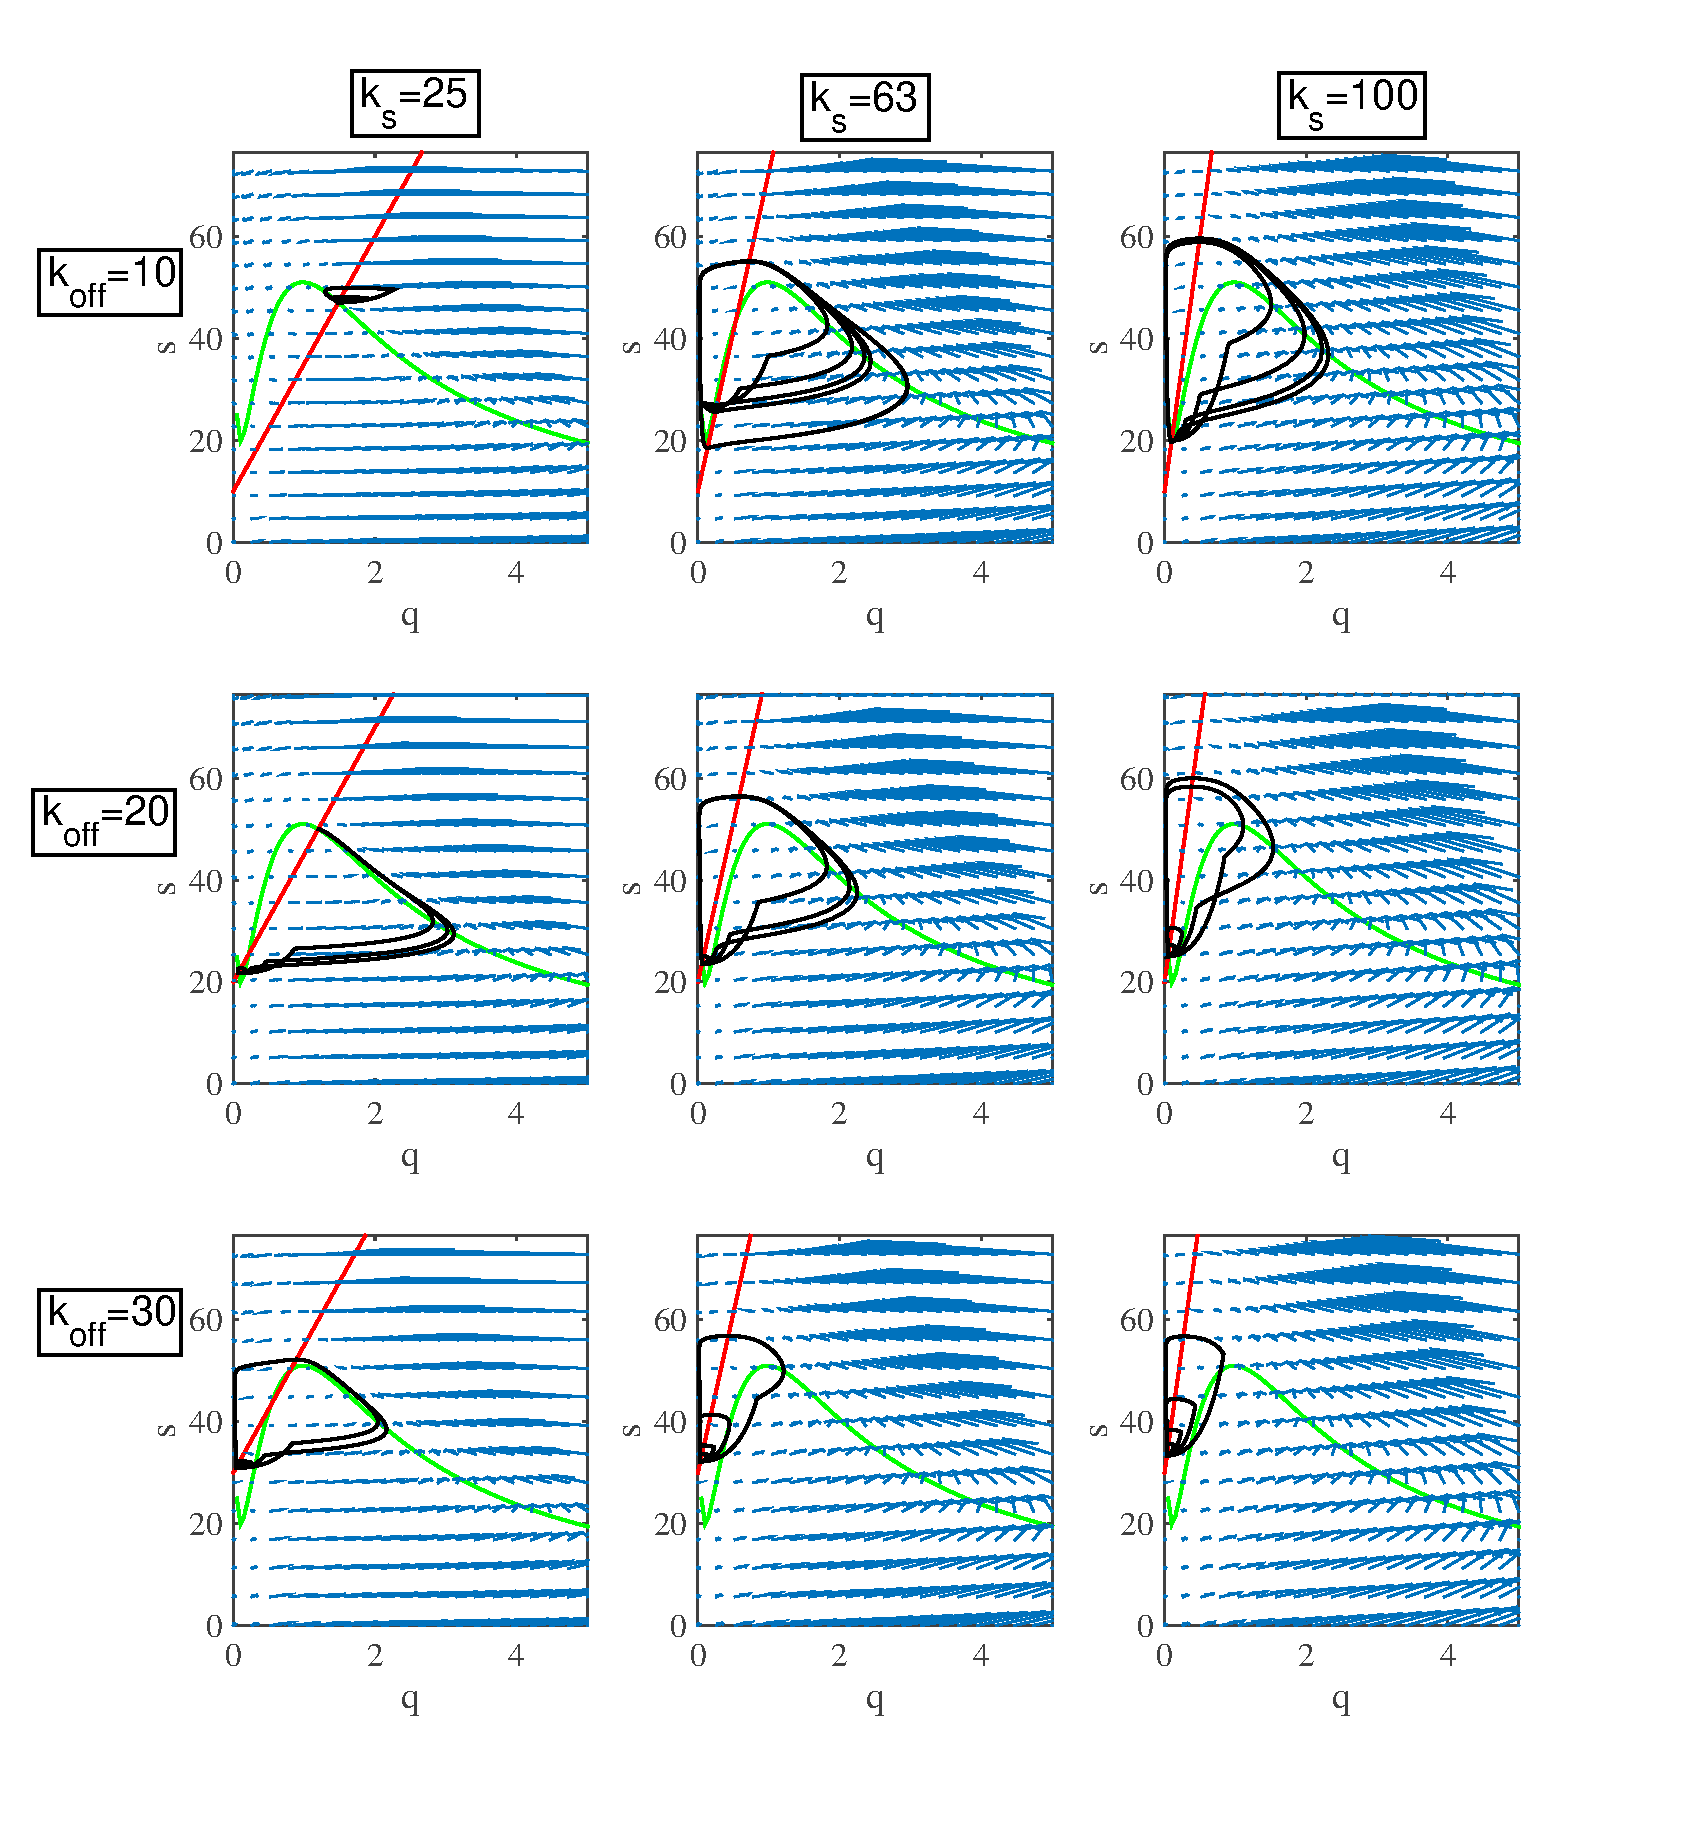
\includegraphics[width=\hsize]{pulse/phase_tester.eps}
	\caption{\label{fig:pulse_test}  Perturbation simulation results plotted on phase planes for a variety of parameters.  }
\end{figure}

The $s_q$ null-cline appears as an inverse relation between $s$ and $q$, with a hump around $q=1$ whose height is dictated by the strength of the $q$ positive feedback, $k_{qq}$.  The $s_s$ null-cline is simply a straight line whose slope is governed by $k_s$.  The dynamical system is only able to attain pulsatile behavior when the $s_s$ null-cline runs parallel and to the left of the hump in the $s_q$ null-cline.  This gives two effective conditions on pulsatility: 1) If $k_{qq}$ isn't much larger than 1, there will not be any hump, and so there cannot be any pulsatility. 2) If $k_s$ and $k_off$

To test this prediction, I implemented an automated search of the model's parameter space.  The test worked by adding perturbations of fixed strength to the equilibrium state, and observing whether the response of the system exceeded the perturbation. As shown in Figure \ref{fig:pulse_test} for a number of simulation parameters, the response function could vary from having just a stable fixed point ( $k_{off}=10$ and $k_s=25$) to having stable oscillations ( $k_{off}=10$ and $k_s=63$) to having pulses ( $k_{off}=20$ and $k_s=63$).  Figure \ref{fig:pulse_test} also shows the null-clines for each case, which can be used to interpret whether pulsation is possible.

\begin{figure}[h!]
	\centering
	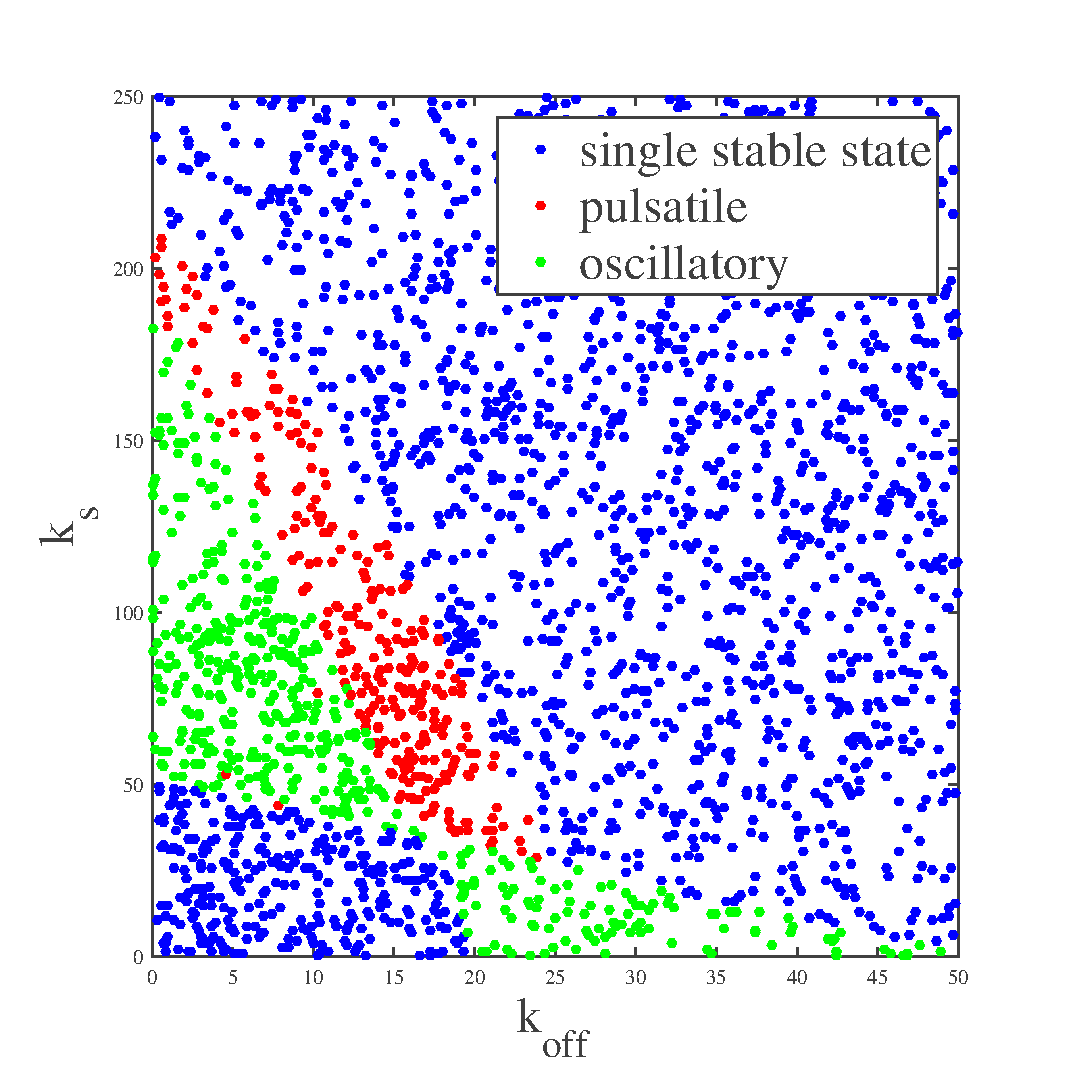
\includegraphics[width=\hsize]{pulse/k_phase.eps}
	\caption{\label{fig:pulse_k_phase}  Phase diagram of for $k_q=1$ and $k_qq=100$.}
\end{figure}

Using this automated system, I was able to generate 1600 simulations and classify them automatically based on the ratio of the magnitude of the perturbation to maximum response (to determine if positive feedback drove excitation) and whether the maximum was attained multiple times (to differentiate pulses and stable oscillations).  This resulted in a phase diagram of the behavior as shown in Figure \ref{fig:pulse_k_phase}, with the three colors indicating the behavior of dynamical systems in that regime.  The size and shape of the pulsing region of phase space was a direct result of the strength of positive feedback ($k_{qq}$)  with stronger feedback allowing more of phase space to permit pulsing and oscillations.

\begin{figure}[h!]
	\centering
	\includegraphics[width=\hsize]{pulse/randomized_simulation.eps}
	\caption{\label{fig:pulse_rando}  }
\end{figure}

Finally, using this understanding of the phases behavior of the system, I implemented a stochastic dynamical equation to test the response to noise.  As indicated in Figure \ref{fig:pulse_rando}, a basal level of noise was able to trigger robust pulses in both Rho and RGA for certain parameters. Taken together this analysis indicated that our biochemical reaction circuit for Rho and RGA feedback could in principle account for the excitable dynamics exhibited in the system.

\section{Simplified model and data fitting}
\subsection{Fitting techniques}
\begin{figure}[h!]
	\centering
	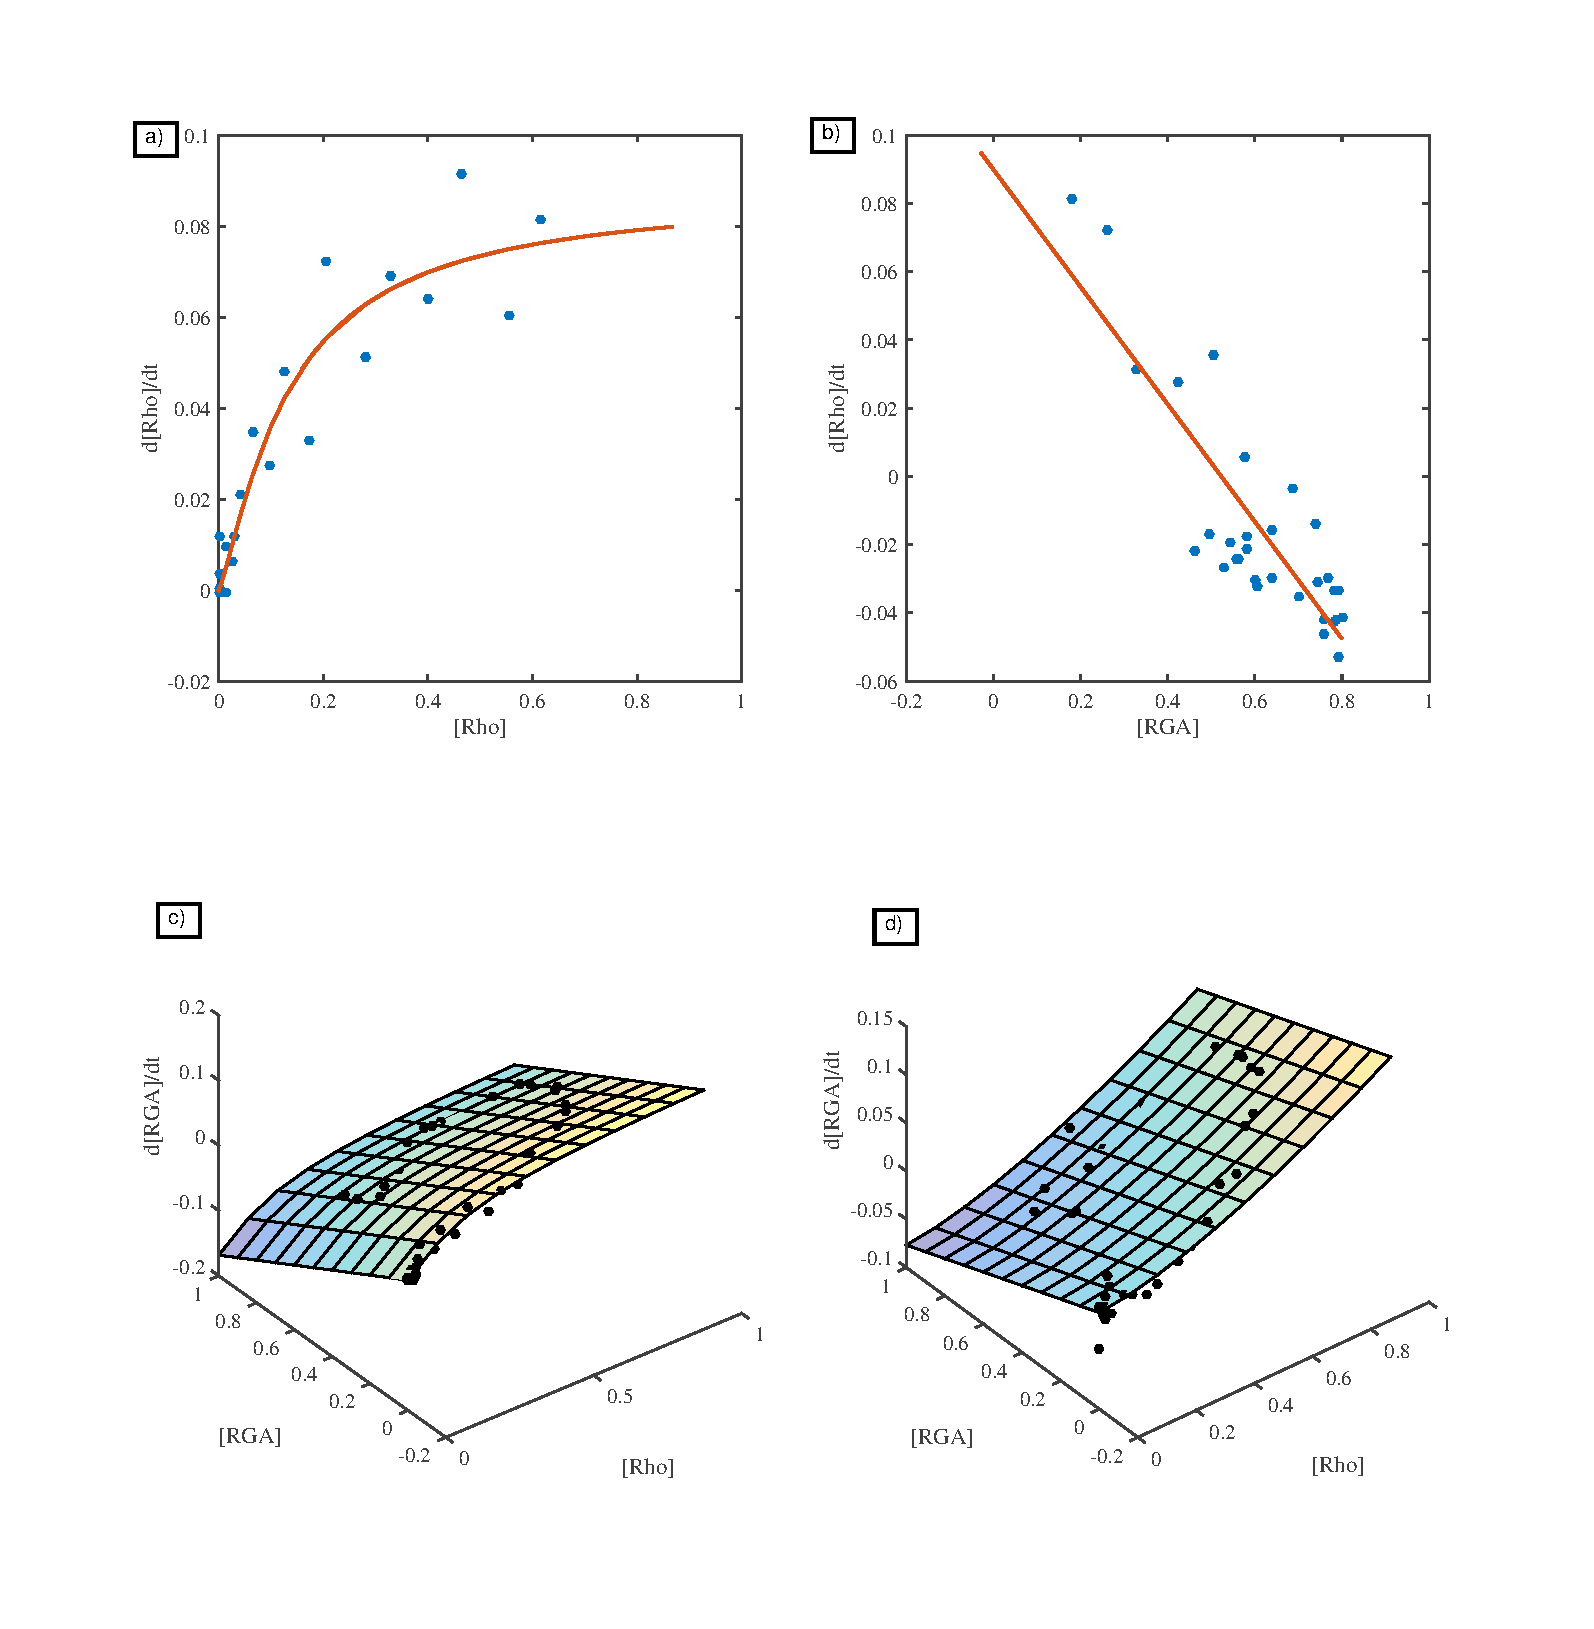
\includegraphics[width=\hsize]{pulse/fitting_plot.eps}
	\caption{\label{fig:pulse_fit}  Multiple methods of fitting.}
\end{figure}

Although this model accounted for the qualitative behavior, we wished to determine whether it could be corroborated by fitting to the data presented in the paper. To experiment with fitting the normalized data, I created a reduced model, where the equilibrium concentration had been renormalized to 0 for both Rho and RGA, and the feedbacks between Rho and RGA are allowed to be non-linear.  

\begin{equation}
	\frac{dq}{d\tau} =\alpha \frac{q^n}{1 +q^n} - s q^k
\end{equation}

\begin{equation}
	\frac{ds}{d\tau} = \beta q^{(m-k)} - s
\end{equation}

These equations resulted in a family of models with different levels of feedback, depending on the values of $n$, $m$, and $k$.  I fit models with a variety of exponents and found that any model with $k\approx0$, $n>1$, and $m\approx2$ gave the best overall agreement with the greatest robustness.  
\begin{figure}[h!]
	\centering
	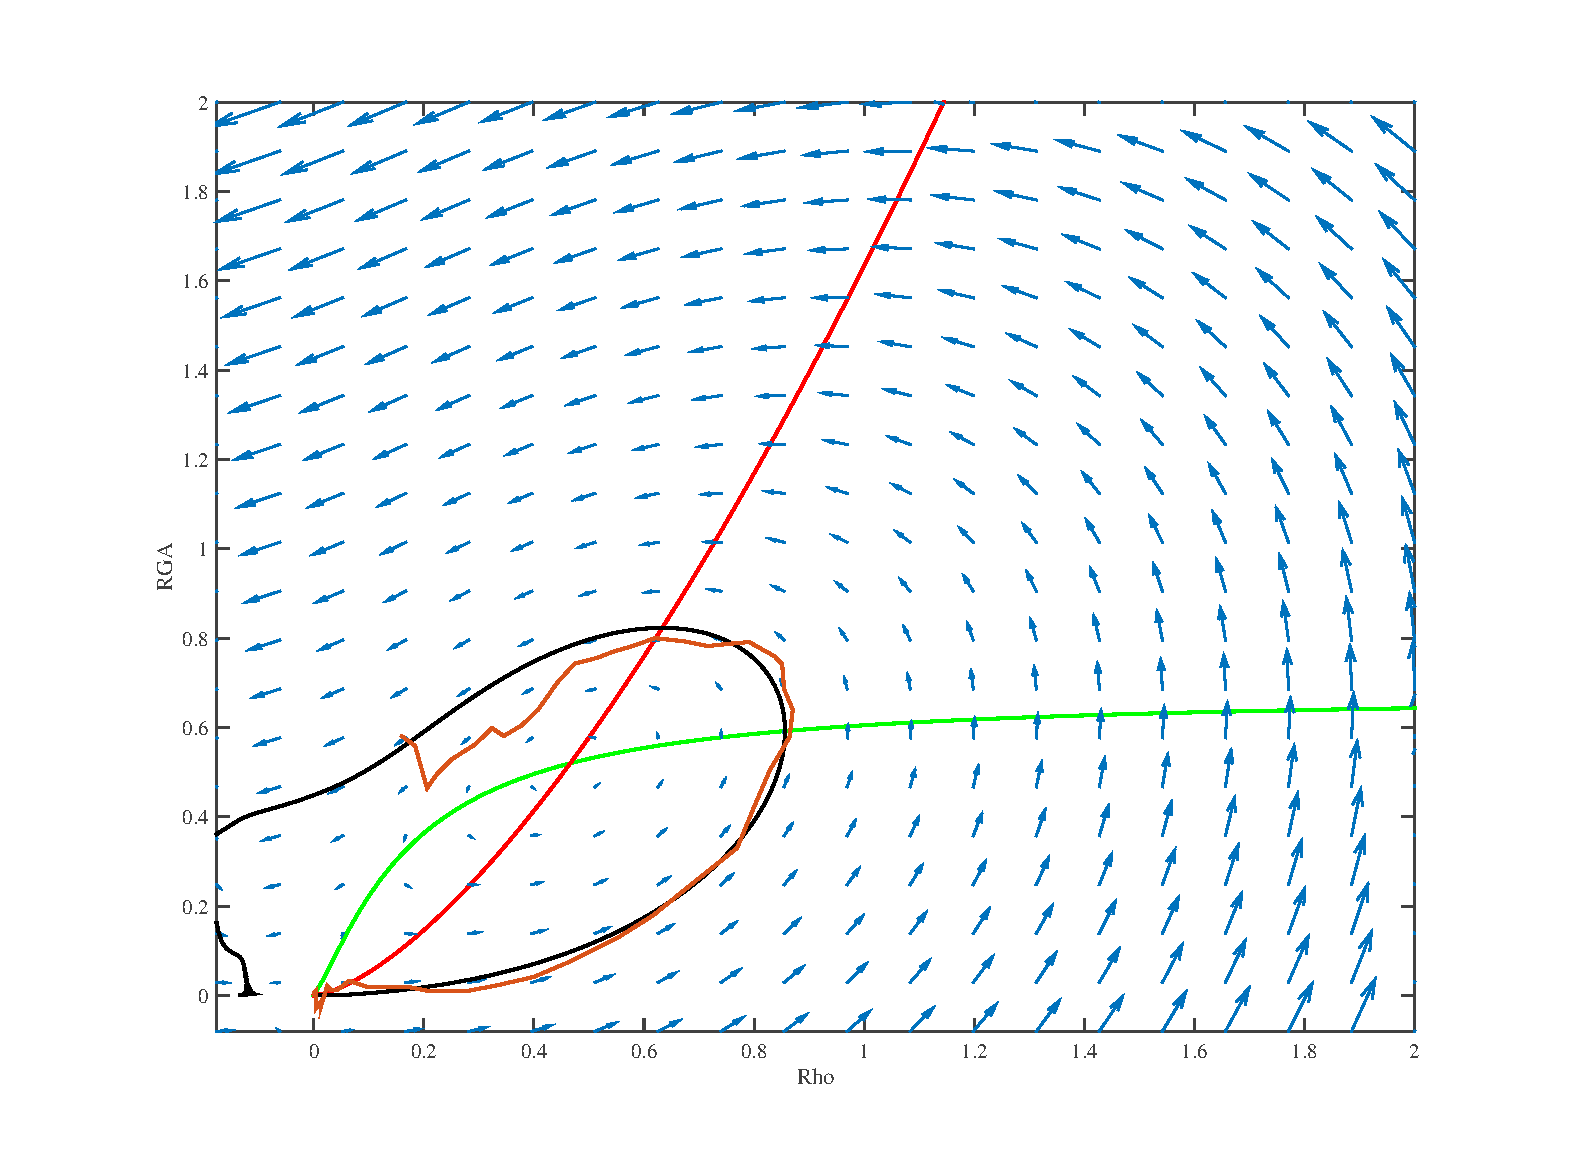
\includegraphics[width=0.45\hsize]{pulse/simple_model_fit_phase.eps}
	\includegraphics[width=0.45\hsize]{pulse/model_profile.eps}
	\caption{\label{fig:pulse_fit_sim}  Simulation results and fitted data for model with $m=2$ and $k=0$. Displaying simulation results and the data used to fit the simulation on a phase plane (left) and as pairs of time plots (right).}
\end{figure}
I used two different methods to fit the Rho and RGA data to determine the most appropriate model parameters.  The first required subsecting the data to fit only datapoints where some terms in the equation were presumably close to constant (Figure \ref{fig:pulse_fit}a,b).  For example, as long as RGA concentration remained relatively small, the equation for Rho could be taken to consist of only the Rho self-feedback function.  The second method allowed fitting all of the data the equations at once (Figure \ref{fig:pulse_fit}c,d).  The second method is clearly more accurate, but it comes at the cost of being slightly more difficult to explain to the lay-biologist.

\begin{figure}[h!]
	\centering
	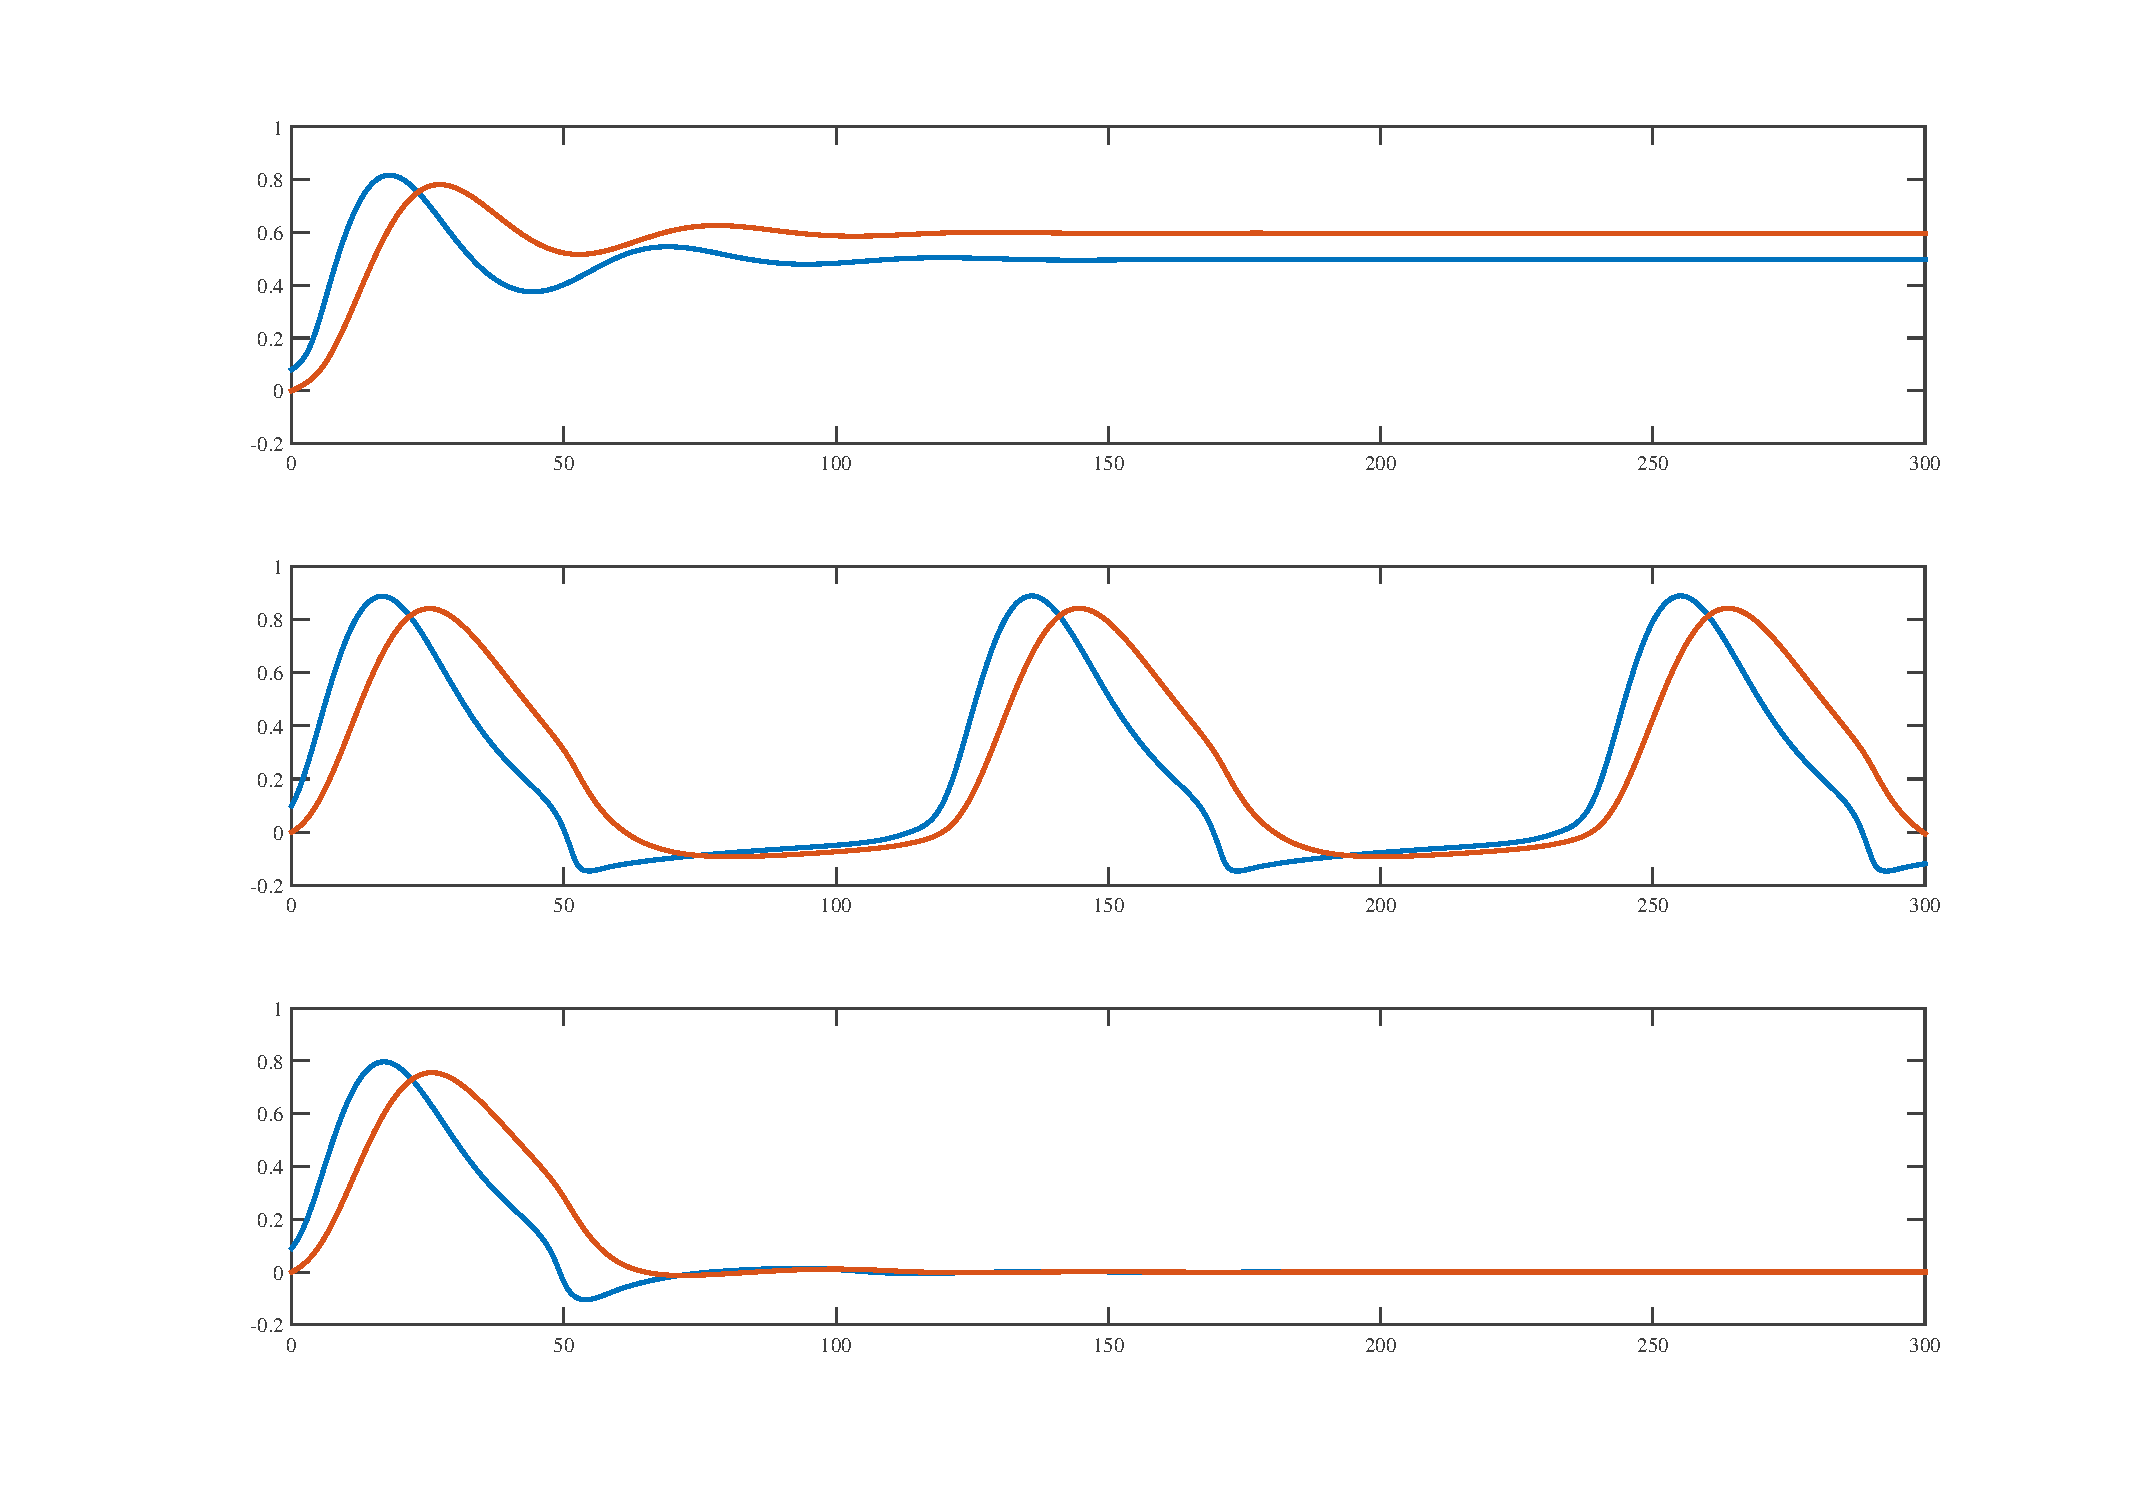
\includegraphics[width=\hsize]{pulse/model_compare.eps}
	\caption{\label{fig:pulse_fit_compare}  Small variation in simulation parameters can have large qualitative effects.}
\end{figure}

The resulting fitted models could then be used to run simulations.  As shown in Figure \ref{fig:pulse_fit_sim}, the models and fitted data were largely indistinguishable relative to the error in the data.  Although the model was quite successful at recapitulating the original data, I found that the resulting models were not necessarily.  For example by changing the value of the parameter $\alpha$ by 25\% and rerunning the fits, I could tune the system from a stable system to pulsatility and into an oscillatory regime (Figure \ref{fig:pulse_fit_compare} ).  Therefore, it appears that this model is not incredibly robust to minor variations in parameters. 


\section{Conclusion}
\begin{figure}[h!]
\centering
\includegraphics[width=\hsize]{pulse/final_fig.png}
\caption{\label{fig:pulse_final}  Final figure as it appears in Robin et al.}
\end{figure}
Ultimately, a model similar to \ref{eqn:rho_1} and \ref{eqn:rga_1} was utilized in the final paper in combination with at the 2D fitting routine outlined in Figure \ref{fig:pulse_fit}c,d.   In short, all models performed fairlt well at describing the qualitative features of the data, but none were very effective at generating a quantitative match with great robustness.    We believe this is indicative of the need to perhaps extend to incorporating spatial effects in driving the dynamics of active material pulses.  Based on the theoretical results of [bois and the other one], we attempted to incorporate our upstream regulatory model into a 1D active fluid.  This ongoing work will hopefully tie together the spatial and temporal interdependencies driving this system into its interesting non-equilibrium state.

